\begin{table*}[t]
\centering
\renewcommand\arraystretch{0.95}
\caption{Case studies on geometric reasoning tasks with \ours-8B trained in \env{}.}
\resizebox{\linewidth}{!}{
    \begin{tabular}{p{1.8cm}p{21cm}}
    % \begin{tabular}{p{2cm}p{18cm}}
       \toprule
       \multicolumn{2}{l}{\textbf{Case Study 1}: Find m $\angle$ R. \textbf{Answer: A}: 58} \\
       % \midrule
        % \bf Q / A & who hosted and won the inagural world cup / Uruguay  \\
        \midrule
        \bf \multirow{6}{*}{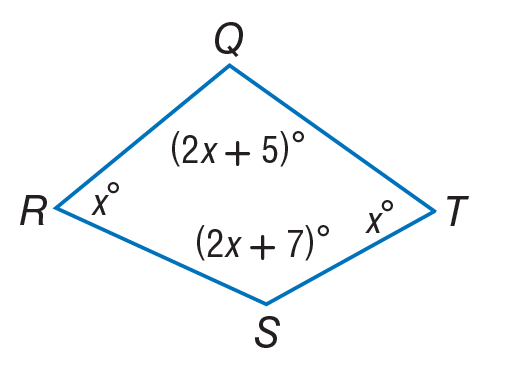
\includegraphics[width=\linewidth]{figure/casestudy/2489_img_diagram.png}} & \textbf{InternVL3-8B-Tool}: \textcolor{blue}{<tool\_call>}\{"tool": "multimath", "task": "solve\_the\_problem", "arguments": \{"image\_url": <image\_url>, "data": \{\textcolor{red}{"image/png": base64, iVBORw0KGgoAAAANSUhEUgAAAOAAAAHCAIAAADYXJpAAAAA3NCSV $\cdots$ (including long base64 image data)}\}\}\textcolor{blue}{</tool\_call>} \hfill \colorbox{red!15}{\textbf{Tool Call Error}: \emph{Invalid Arguments}. (\ding{56})} \\
        & \textbf{\ours}: \textcolor{blue}{<tool\_call>}\{"tool": "gllava", "task": "solve", "arguments": "Find m $\angle R$ from the diagram: a diamond-shaped quadrilateral with vertices R (left), Q (top), T (right), S (bottom). Angles labeled: at $R = x^\circ$, at $T = x^\circ$, at $Q = (2x+5)^\circ$, at $S = (2x+7)^\circ$."\}.\textcolor{blue}{</tool\_call>} \hfill \colorbox{green!15}{\textbf{Tool Call}: \emph{Correct} (\ding{51})} \\
        \midrule
        \multicolumn{2}{p{23cm}}{\textbf{Case Study 2}: As shown in the figure, in $\odot O$, $AB$ is a diameter and $CD$ is a chord. $AB \perp CD$, with the foot of the perpendicular at point $E$. Connect $CO$ and $AD$. If $\angle BOC = 30^\circ$, then the degree measure of $\angle BAD$ is ( ). \textbf{Answer: 15$^\circ$}} \\
        \midrule
        \bf \multirow{6}{*}{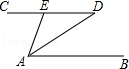
\includegraphics[width=\linewidth]{figure/casestudy/102.png}}  & \textbf{InternVL3-8B-Tool}: $\cdots$\textasciigrave\textasciigrave\textasciigrave output $\cdots$Step 12 (Property of isosceles triangle): $\angle BAD = \angle OAD$. Answer: $\angle BAD = 15^\circ$.\textasciigrave\textasciigrave\textasciigrave \textcolor{blue}{<think>} Alright, \textcolor{red}{let's tackle this geometry problem step by step}. $\cdots$ But according to the tool output, the answer is 15 degrees, which is option D. \textcolor{red}{But my computation also says the answer is 52.5 degrees. So the answer is closer to C}. \textcolor{blue}{</think>}$\cdots$ \hfill \colorbox{red!15}{\textbf{Correct Tool, Wrong Reasoning}: \emph{Incorrect reasoning to answer.}. (\ding{56})}\\
        & \textbf{\ours}: $\cdots$ \textasciigrave\textasciigrave\textasciigrave output $\cdots$Step 12 (Property of isosceles triangle): $\angle BAD = \angle OAD$. Answer: $\angle BAD = 15^\circ$.\textasciigrave\textasciigrave\textasciigrave\textcolor{blue}{<think>} \textcolor{green!50!black}{$\cdots$Based on the previous verification and tool output, I can analyze and provide the answer of $15^\circ$.}\textcolor{blue}{</think> <answer>}15$^\circ$\textcolor{blue}{</answer>}. \hfill \colorbox{green!15}{\textbf{Reasoning}: \emph{Correct} (\ding{51})} \\
        \midrule
        \multicolumn{2}{p{23cm}}{\textbf{Case Study 3}: $AB || CD$. Line $EF$ intersects $AB$ at point $E$ and intersects $CD$ at point $F$. $EG$ bisects $\angle BEF$ and intersects $CD$ at point $G$. If $\angle 1 = 50^\circ$, then $\angle 2$ equals ( ). Choices:A: $50^\circ$B: $60^\circ$C: $65^\circ$D: $90^\circ$. \textbf{Answer: C: 90$^\circ$.}} \\
        \midrule
        \bf \multirow{7}{*}{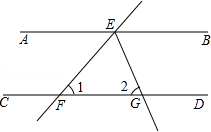
\includegraphics[width=\linewidth]{figure/casestudy/1.png}} & \textbf{\ours}: \textcolor{blue}{<think>} $\cdots$ \textcolor{green!50!black}{ChartMoE is appropriate because it is designed to analyze structured geometric diagrams, accurately reading angle labels, identifying parallel-line configurations, and aligning textual annotations with diagram elements. I will have it parse the diagram to confirm $AB||CD$, locate the transversal EF and the points E, F, G, and verify that EG bisects $\angle BEF$ while intersecting CD at G.} By interpreting the angles formed at E relative to BE and FE and using the parallel-line angle relations (corresponding, alternate interior, and consecutive interior angles), ChartMoE will relate $\angle 1$ to the angle between BE and EG, propagate the bisector relation to $\angle BEF$, and then deduce the measure of $\angle 2$ at the intersection of EF and CD from the resulting angle measures. Finally, it will align that computed value with the provided choices. Therefore, I will call chartmoe now.\textcolor{blue}{</think><tool\_call>}\{"tool": "chartmoe", "task": "analyze"\}\textcolor{blue}{</tool\_call>} $\cdots$ \hfill \colorbox{green!15}{\textbf{New Tool Selection}: \emph{Expected G-LLaVA but got ChartMoE.} (\ding{51})}\\
        \midrule
        \multicolumn{2}{p{23cm}}{\textbf{Case Study 4}: Find X Z. \textbf{Answer: D: 34.}} \\
        \midrule
        \bf \multirow{16}{*}{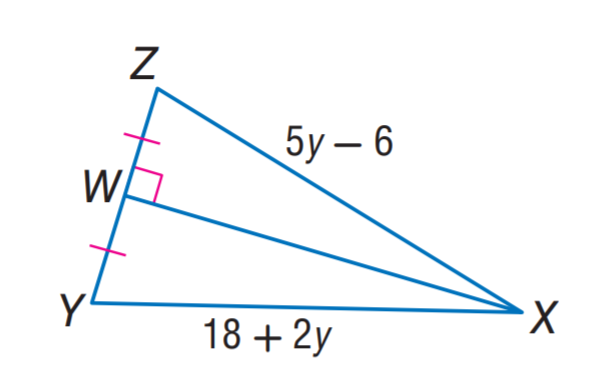
\includegraphics[width=\linewidth]{figure/casestudy/2430_img_diagram.png}} & \textbf{InternVL3-8B-Tool}: \textcolor{blue}{<tool\_call>}\{"tool": "multimath", "task": "Solve the problem", "arguments": \{"image": "<image>", "question": "Find X Z. $\cdots$"\}\}\textcolor{blue}{</tool\_call>}\textasciigrave\textasciigrave\textasciigrave output $\cdots$ Step 5 (Simplify the equation): $XZ^2 = 29y^2 + 12y + 360.$\textbackslash nAnswer: \textbackslash boxed\{$29y^2 + 12y + 360$\}\textasciigrave\textasciigrave\textasciigrave\textcolor{blue}{<think>} $\cdots$ But as we saw earlier, this leads to a quadratic with no real solutions.\textbackslash n \textcolor{red}{Wait, maybe I made a mistake in the tool output. Let me double-check the steps: \textbackslash n Step 3: $XZ^2 = (5y - 6)^2 + (18 + 2y)^2 = 25y^2 - 60y + 36 + 324 + 72y + 4y^2 = 29y^2 + 12y + 360$. That seems correct.}\textbackslash n $\cdots$ Step 5: Simplify the equation: $XZ^2 = 29y^2 + 12$\textcolor{blue}{</think><answer>} \textbackslash boxed\{C\}.\textcolor{blue}{</answer>} \hfill \colorbox{red!15}{\textbf{Tool Output Error}: \emph{Incorrect reasoning to answer.}. (\ding{56})}\\
        & \textbf{InternVL3-8B-Reasoning}: <think> Alright, let's tackle this problem step by step. First, I notice that triangle WYZ is a right triangle because it has a right angle at W. $\cdots$ Using the Pythagorean theorem again:\textbackslash n$XZ^2 = WZ^2 + XY^2$\textbackslash n$XZ^2 = 34^2 + 34^2$, $XZ^2=2312$, $XZ=\sqrt{2312}=34*\sqrt{2}$\textbackslash n Therefore, the length of XZ is $34\sqrt{2}$.\textbackslash n</think>\textbackslash n<answer>$34\sqrt{2}$</answer>" \hfill \colorbox{red!15}{\textbf{No Tool-use}: \emph{Insufficient capability to answer.}. (\ding{56})}\\
        & \textbf{\ours}: \textcolor{blue}{<think>} $\cdots$ \textcolor{green!50!black}{Multimath is appropriate because} $\cdots$ I will read from the image that $WX\perp ZX$ $\cdots$. \textcolor{green!50!black}{Multimath will translate these visual relations into algebraic constraints}, $\cdots$. \textcolor{blue}{</think><tool\_call>}\{"tool": "multimath", "task": "solve"\}\textcolor{blue}{</tool\_call>}\textasciigrave\textasciigrave\textasciigrave output $\cdots$ Step 10 (Calculate the value of XZ): $XZ = 18 + 2y = 18 + 2(\frac{6}{5}) = 18 + \frac{12}{5} = \frac{90}{5} + \frac{12}{5} = \frac{102}{5} = 20.4$. \textasciigrave\textasciigrave\textasciigrave \textcolor{blue}{<think>} Looking at the tool's solution, it set up the equation $25y^2 - 60y + 36 = 0$ and solved to get $y = 6/5$. Let me verify this step by step. $\cdots$ \textcolor{green!50!black}{Wait, let me check if this makes sense geometrically.} $\cdots$ Actually, if the tick marks indicate equal segments, shouldn't we have $5y - 6 = 18 + 2y$? Let me solve this: $5y - 6 = 18 + 2y 3y = 24 y = 8$ With $y = 8$, let's calculate XZ. If $XZ = 18 + 2y$, then: $XZ = 18 + 2(8) = 18 + 16 = 34$. \textcolor{green!50!black}{Hmm, that's different from the tool's answer of $20.4$. Let me reconsider.} $\cdots$ \textcolor{green!50!black}{The tool calculated 20.4, but based on the equal segment marks, the answer is $34$.}\textcolor{blue}{</think><answer>}$34$\textcolor{blue}{</answer>}" \hfill \colorbox{green!15}{\textbf{TIR}: \emph{correct} (\ding{51})} \\
       \bottomrule
    \end{tabular}
%\end{center}
}
 % \vspace{-1ex}
	\label{tab:case_study}
\end{table*}
